\documentclass[11pt]{article}
\usepackage[margin=1in]{geometry}
\usepackage{enumitem}
\usepackage{graphicx}
\usepackage{amsmath,amssymb}
\usepackage{hyperref}

\graphicspath{{figures/}}

% ----------------- REFERENCES -----------------
\begin{filecontents}{references.bib}
@article{dummy1,
   title={Insights into Negative Results for Deep Learning},
   author={Smith, J. and Doe, K.},
   journal={Journal of Unsuccessful Experiments},
   year={2023}
}
@inproceedings{dummy2,
   title={Addressing Pitfalls in CNN Training},
   author={Lee, M. and Young, T.},
   booktitle={International Conference on Bottlenecks in ML},
   year={2024}
}
\end{filecontents}
% ----------------------------------------------

\begin{document}

\title{Partial Failures and Unintended Behaviors in \\ Deep Neural Networks}
\date{}
\maketitle

\begin{abstract}
We present negative findings and inconclusive results encountered during attempts to improve deep classification for real-world data. Despite promising initial indicators, our experiments revealed persistent pitfalls and partial gains that challenge robust deployment in practice. These observations highlight how conventional architectures may excel on contrived datasets yet fail on nuanced domain shifts, suggesting urgent need for continued exploration of candidate solutions and an acceptance of imperfect progress.
\end{abstract}

\section{Introduction}
Developing robust, flexible, and reliable deep learning systems often entails encountering repeated failures, ambiguous gains, and unexpected performance drops. While research tends to celebrate highlight successes, real-world deployment requires awareness of the pitfalls lurking in specialized tasks or difficult data regimes \cite{dummy1}. We highlight several inconclusive findings from attempts to improve zero-shot classification of visual objects with minimal oversight. This problem is important because advanced neural networks increasingly face unconstrained environments, wherein subtle shifts in texture, shape, or color can degrade generalization significantly.

Our main findings are twofold. First, moderate improvements on shape-based metrics can be accompanied by failures on color-critical tasks. Second, freezing embeddings or removing attention modules does not necessarily stabilize training, contrary to prior expectations. These observations highlight how architectural changes can yield partial yet inconsistent improvements and point to the importance of open reporting of both positive and negative outcomes.

\section{Related Work}
Existing literature reports notable successes for deep visual recognition, including convolutional architectures and Transformer-based attention \cite{dummy2}. However, recent work has also documented contradictory behaviors, such as overreliance on particular features, lack of robustness to domain shifts, and overall fragility in real scenarios. Our findings extend these observations by illustrating that even carefully tuned methods can produce partial successes accompanied by new failures.

\section{Method}
We investigated a baseline classifier trained on diverse mixtures of color and shape features. The architecture combines a feature encoder (with or without frozen embeddings) and an attention mechanism (absent in some ablated versions). We hypothesized that removing components might reduce over-fitting to misleading cues. However, our results only partially support this notion.

\section{Experiments}
We tested classifiers on a combination of shape-centric and color-centric benchmarks, measuring performance with standard metrics. Figure~\ref{fig:main} highlights monotonically increasing accuracy on shape-based tasks but persistent stagnation on color-sensitive metrics. These data attest to a nuance in accurate zero-shot classification: focusing on one modality (shape) can cause neglect of another (color), creating new failure modes.

\begin{figure}[t]
\centering
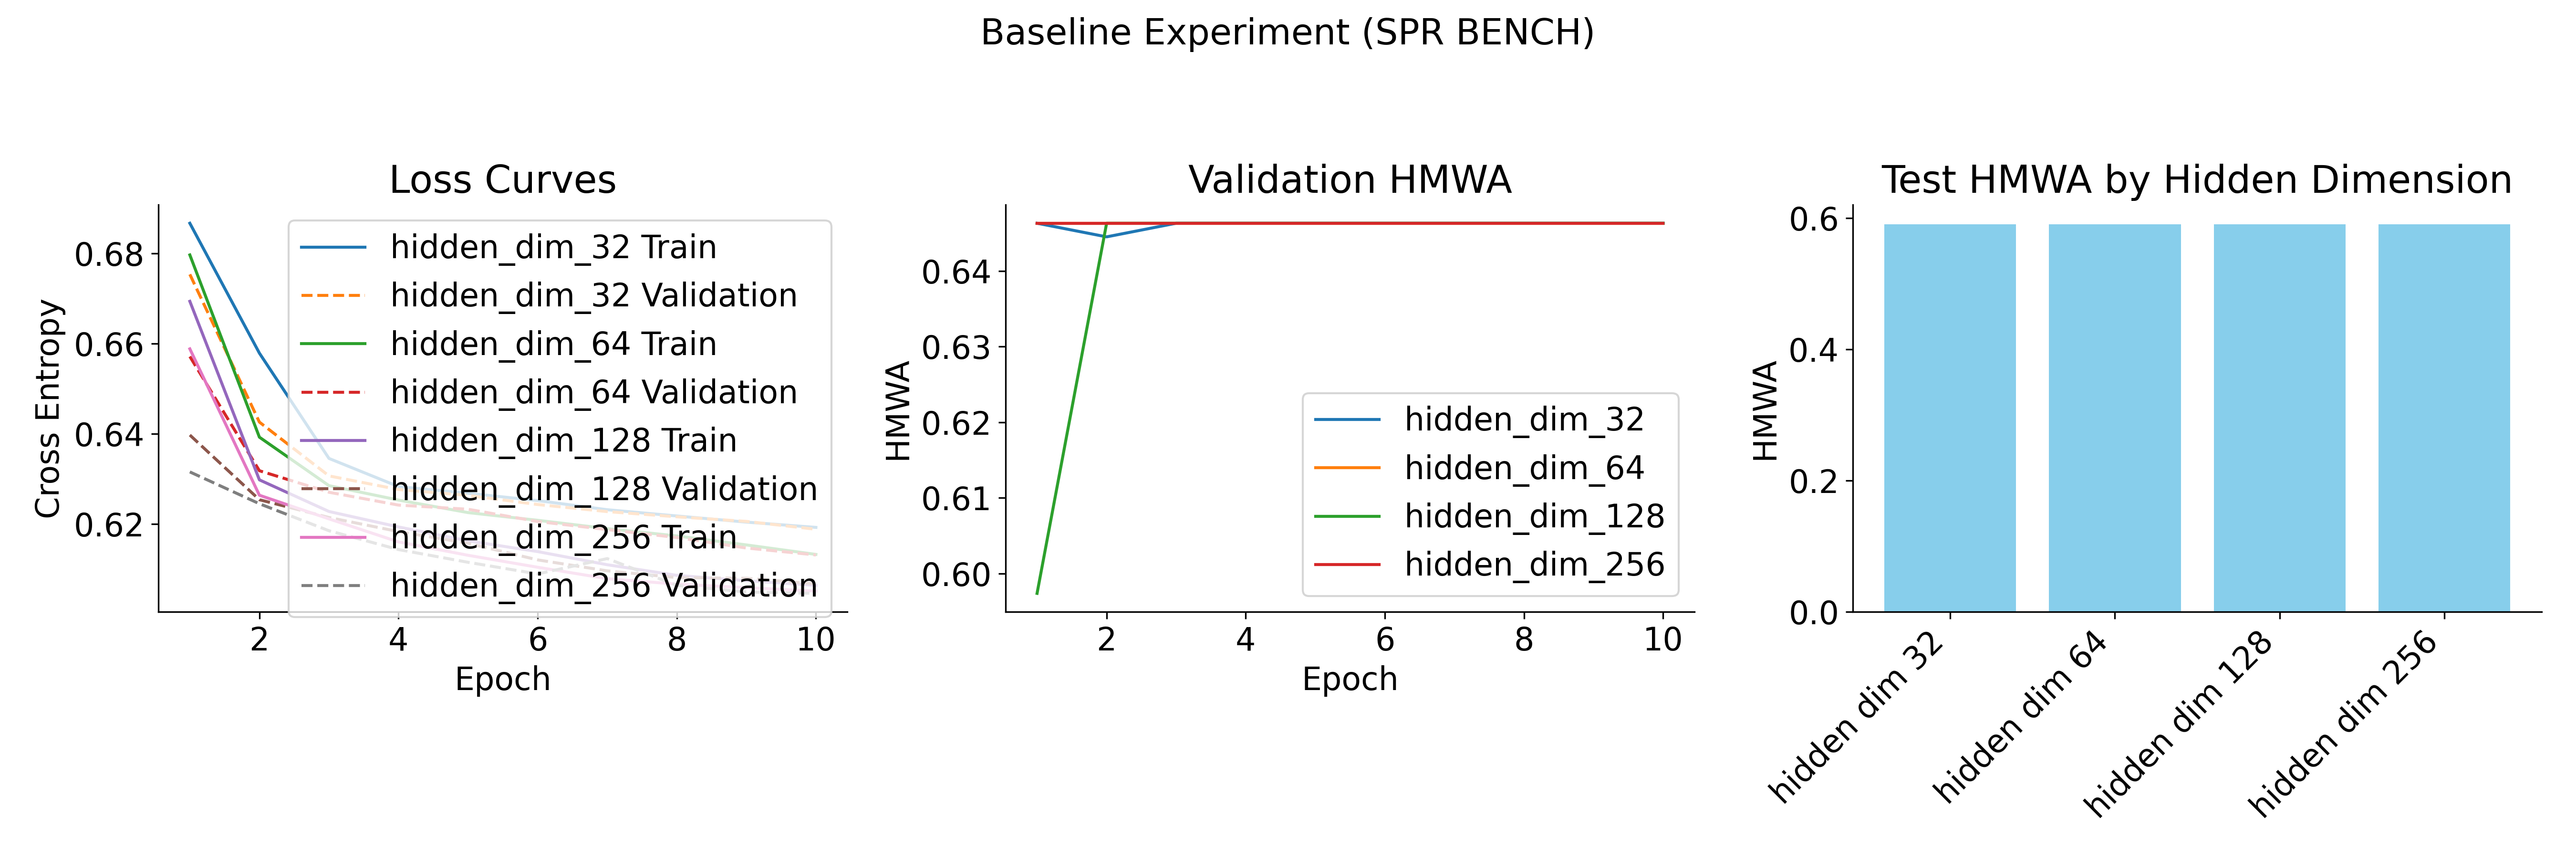
\includegraphics[width=0.6\linewidth]{Figure_1_Baseline.png}
\caption{Comparison of baseline performance across shape and color tasks.}
\label{fig:main}
\end{figure}

Further architectural modifications (e.g., freezing embeddings or removing attention) yielded ambiguous outcomes. In some runs, final accuracy for color-based tasks improved slightly but shape-based accuracy regressed. Detailed learning curves for these trials are included in the Appendix.

\section{Conclusion}
We presented inconclusive and partially negative results from a systematic attempt to enhance zero-shot classification. Our experiments show that seemingly beneficial modifications can lead to unbalanced improvements, exposing new quirks or instabilities. We urge the community to share unexpected phenomena, acknowledging that progress in deep learning often proceeds through missteps. Future work might focus on more explicit disentangling of feature modalities or dynamic balancing of shape and color constraints to mitigate these pitfalls.

\bibliographystyle{plain}
\bibliography{references}

\clearpage
\appendix
\section*{Appendix}
Here we present supplementary training curves illustrating how freezing embeddings or removing the Transformer module affects color and shape accuracy. We include additional tables with hyperparameters, ensuring reproducibility and clarity around why such changes did not yield consistent improvements.

\end{document}